\documentclass[oneside,reqno]{amsart}
\setlength{\textwidth}{\paperwidth}\addtolength{\textwidth}{-2in}\calclayout
\usepackage[utf8]{inputenc}
\usepackage{enumitem}
\usepackage{tikz}
\usepackage{minted}\newminted{python3}{frame=lines}
\usepackage{booktabs}
\usepackage{etoolbox}
\makeatletter
\patchcmd{\@sect}{%
   \ignorespaces#8\unskip\@addpunct.}{\ignorespaces#8\unskip}{}{}
\makeatother
\allowdisplaybreaks[1]

\DeclareMathOperator{\var}{var}
\DeclareMathOperator{\cov}{cov}
\DeclareMathOperator{\corr}{corr}
\DeclareMathOperator{\tr}{tr}
\DeclareMathOperator{\diag}{diag}
\DeclareMathOperator{\rank}{rank}
\let\vec\relax\DeclareMathOperator{\vec}{vec}
\let\vech\relax\DeclareMathOperator{\vech}{vech}
\newcommand{\eps}{\varepsilon}
\newcommand{\ups}{\upsilon}

\theoremstyle{definition}
\newtheorem{prob}{Problem}
\renewcommand*{\proofname}{Solution}
\setlist[enumerate]{label={(\roman*)}}


\title{ECON 706: Problem Set 1}
\author{Daniel Pfeffer}
%------------------------------------------------------------------------------
\begin{document}
\maketitle

\begin{prob}
Prove that for a weakly stationary process, $|\gamma(\tau)| \leq \gamma(0)$ for all $\tau$.
\end{prob}

\begin{proof}
Let $\{y_t\}$ be a weakly stationary process, and without loss of generality assume the mean of $y_t$ is zero for all $t$. Then, by the Cauchy-Schwartz inequality, 
\[
	| \gamma(\tau) | = E y_t y_{t-\tau} \leq \sqrt{E y_t^2 E y_{t-\tau}^2} \leq \gamma(0).
\]
\end{proof}

\begin{prob}
Consider an AR(2) process
\end{prob}

\begin{enumerate}
\item
Characterize the conditions for stationarity. 
\begin{proof}
Write the AR(2) process as $(1 - \phi_1 L -  \phi_2 L^2)y_t =  \eps_t$ where $\eps_t \sim WN(0, \sigma^2)$, and consider the characteristic polynomial $\phi(z) = 1 - \phi_1 z - \phi_2 z^2$. Then the $\{y_t\}$ process is non-explosive if the characteristic equation 
\[
	z^2 -\phi_1 z - \phi_2 = 0
\]
has root pairs $(z_1,z_2)$ outside the locus $\{z : |z| > 1\}$ called the unit circle:
\[
	\left| \frac{-\phi_1 \pm \sqrt{\phi_1^2 + 4\phi_2}}{2} \right| > 1.
\]
From this restriction on the roots of $\phi(z)=0$ we can deduce restrictions on the autoregressive parameters. Substituting these roots into the characteristic polynomial for the coefficients gives the factorization 
\[
	\phi(z) = (1- z_1^{-1}z)(1- z_2^{-1}z).
\]
Here, it is identically the case that $\phi(z_1) = \phi(z_2) = 0$. Next rewrite the AR(2) process with the lag operator using this factorization: $(1- z_1^{-1}L)(1- z_2^{-1}L)y_t = \eps_t$, which implies that $\phi_1 = z_1^{-1}+ z_2^{-1}$ and $\phi_2 =-(z_1z_2)^{-1}$. Then, together with the restriction that $|z_1| > 1$ and $|z_2|>1$, we obtain the values for which $\{y_t\}$ is non-explosive:
\[
	\phi_1 + \phi_2 < 1, \qquad \phi_2 - \phi_1 < 1, \qquad |\phi_2| < 1,
\]
a convex set in parameter space. 
\end{proof}
\item
Assuming stationarity, derive its Wold representation, i.e., the coefficients $\psi_i$ for $i=1,2,\dotsc$.
\begin{proof}
To obtain the Wold representation of an AR(2) process, invert then autoregressive lag polynomial using the partial fraction decomposition:
\[
	\frac{1}{(1-\lambda_1 L ) (1-\lambda_2 L)} = \frac{c_1}{(1-\lambda_1 L )} + \frac{c_2}{(1-\lambda_2 L)} = \frac{c_1(1-\lambda_2 L) + c_2 (1-\lambda_1 L)}{(1-\lambda_1 L ) (1-\lambda_2 L)}
\]
where $c_1$ and $c_2$ are coefficients to be determined. We require that $c_1 + c_2 = 1$ and $\lambda_2 c_1 + \lambda_1 c_2 = 0$. Hence, the solution is 
\[
	c_1 = \frac{\lambda_1}{\lambda_1 - \lambda_2}, \quad c_2 = \frac{-\lambda_2}{\lambda_1 - \lambda_2}.
\]
Substituting this solution into the partial fraction decomposition gives  
\[
	\frac{1}{(1-\lambda_1 L ) (1-\lambda_2 L)} = 	\frac{\lambda_1}{(\lambda_1 -\lambda_2) (1-\lambda_1 L)} 
+ \frac{\lambda_2}{(\lambda_2 -\lambda_1) (1-\lambda_2 L)}.
\]
Now apply this expression for the inverted lag polynomial operator to our AR(2) process to obtain the Wold representation:
\begin{align*}
	y_t &= \frac{\lambda_1}{\lambda_1 -\lambda_2}  \sum_{i=0}^\infty \lambda_1^i\eps_{t-i} + \frac{\lambda_2}{\lambda_2 -\lambda_1} \sum_{i=0}^\infty \lambda_2^i  \eps_{t-i} \\
	&= \sum_{i=0}^\infty \left(\frac{\lambda_1}{\lambda_1 -\lambda_2} \lambda_1^i +\frac{\lambda_2}{\lambda_2 -\lambda_1}\lambda_2^i \right) \eps_{t-i} \\
	&= \sum_{i=0}^\infty \left(c_1\lambda_1^i +c_2 \lambda_2^i \right) \eps_{t-i} = \sum_{i=0}^\infty \psi_i \eps_{t-i},
\end{align*}
where $\psi_i = c_1 \lambda_1^i + c_2 \lambda_2^i$, for  $i = 0,1,2,\dotsc$.
\end{proof}

\item
Verify that $\psi_0=1$.

\begin{proof}
To verify that $\psi_0=1$, first note that $\psi_0 = c_1 \lambda_1^0 + c_2 +\lambda_2^0 = c_1 + c_2$, and then substitute in the expressions for $c_1$ and $c_2$ derived in (b) to obtain
\[
	\psi_0 = \frac{\lambda_1}{\lambda_1 - \lambda_2} + \frac{-\lambda_2}{\lambda_1 - \lambda_2} = \frac{\lambda_1- \lambda_2}{\lambda_1 - \lambda_2} =1,
\]
the desired result.
\end{proof}

\item
Verify that the square summability conditional holds, i.e., $\sum_{i=0}^\infty \psi_i^2 < \infty$.

\begin{proof}
Write the infinite sum 
\begin{align*}
	\sum_{i=0}^\infty \psi_i^2 &= \sum_{i=0}^\infty \left(c_1\lambda_1^i +c_2 \lambda_2^i \right)^2 = c_1^2 \sum_{i=0}^\infty \lambda_1^{2i} + c_2^2 \sum_{i=0}^\infty \lambda_2^{2i} + c_1 c_2 \sum_{i=0}^\infty (\lambda_1\lambda_2)^{2i}.
\end{align*}
We know from the stationarity conditions derived in (i) that $\lambda_1$ and $\lambda_2$ have modulus less than unity, which implies that each term is a convergent geometric series. Hence $\sum_{i=0}^\infty \psi_i^2 < \infty$.
\end{proof}
\end{enumerate}

\begin{prob}
Is the following process stationary?
\begin{equation}\label{eq:q3-process}
	y_t = 0.5 y_{t-1} + 0.9 y_{t-2} - 0.1 y_{t-3} + 0.3 y_{t-4} + 0.5 \eps_{t-1} + \eps_t
\end{equation}
\end{prob}

\begin{proof}
First rewrite the process in lag operator notation as
\[
	(1-0.5L - 0.9 L^2 + 0.1 L^3 - 0.3 L^4)y_t = (1+0.5 L)\eps_t.
\]
Notice that we can factor autoregressive operator and moving average operator as 
\begin{align*}
	\phi(L) &= (1-0.5L - 0.9 L^2 + 0.1 L^3 - 0.3 L^4) = -0.1 (L + 2) (3L^3 - 7L^2 + 5L - 5) \\
	\theta(L) &= (1+0.5 L) = 0.5 (L+2).
\end{align*}
which have a common factor $(L+2)$ and therefore a redundant parameter. So we can rewrite this process as an AR(3) model of the form $-0.1(3L^3 - 7L^2 + 5L - 5)y_t = 0.5 \eps_t$. This process is stationary if the roots of the characteristic polynomial
\[
	\phi(z) = -0.3z^3 + 0.7z^2  - 0.5z + 0.5.
\]
are outside the unit circle. Factoring the characteristic equation as 
\[
	-0.3 (z - 1.91744) (z^2 - 0.415894 z + 0.869215) = 0
\]
immediately gives the real root $z_1 = 1.91744$, which is outside the unit circle. To obtain the other two roots, use the quadratic equation 
\[
	z_2, z_3 = \frac{0.415894 \pm \sqrt{(-0.415894)^2 + 4(0.869215)}}{2}
\] 
which gives the complex roots (that occur in a complex conjugate pair) as $z_2 = 0.207947 + 0.908831 i$ and $z_3= 0.207947 - 0.908831 i$. Their modulus is $0.932317 < 1$, and so the process is not stationary. 
\end{proof}

\begin{prob}
Consider 
\begin{align*}
	x_t &= \phi_1 x_{t-1} + \phi_2 x_{t-2} + \phi_3 x_{t-3} + \eps_t \\
	y_t &= \theta_1 \eps_1 + \theta_2 \eps_{t-2} + \eps_t \\
	z_t &= \phi_1 z_{t-1} + \phi_2 z_{t-2} + \phi_3 z_{t-3} + \theta_1 \eps_t + \theta_2 \eps_{t-2} + \eps_t.
\end{align*}
Take $(\phi_1, \phi_2, \phi_3, \theta_1, \theta_2) = (0.6, 0.2, 0.1, 0.5, -0.2)$ and assume $\eps_t \sim N(0,1)$.
\end{prob}

\begin{enumerate}
\item
Starting from arbitrary initial values, simulate a plot of a series of $T=10000$ realizations for each process. 
\begin{proof}
Below is the code used to simulate the processes and plot the resulting series. Figure \ref{4a} contains simulated series for the $x_t$, $y_t$ and $z_t$ processes, respectively.
\begin{python3code}
import numpy as np
import matplotlib.pyplot as plt
from statsmodels.graphics.tsaplots import plot_acf, plot_pacf

# Simulate the series
np.random.seed(42)
T = 10000
eps = np.random.normal(0,1,size=T)
x, y, z = np.empty_like(eps), np.empty_like(eps), np.empty_like(eps) 
for t in range(T):
    x[t] = 0.6*x[t-1] + 0.2*x[t-2] + 0.1*x[t-3] + eps[t]
    y[t] = 0.5*eps[t-1] - 0.2*eps[t-2] + eps[t]
    z[t] = 0.6*z[t-1] + 0.2*z[t-2] + 0.1*z[t-3]\
           + 0.5*eps[t-1] - 0.2*eps[t-2] + eps[t]

# Plot results           
plt.figure(figsize=(12,4))

plt.subplot(131)
plt.plot(x)
plt.ylabel('$x_t$')

plt.subplot(132)
plt.plot(y)
plt.ylabel('$y_t$')

plt.subplot(133)
plt.plot(z)
plt.ylabel('$z_t$')

plt.tight_layout()
plt.show()         
\end{python3code}
 
\begin{figure}
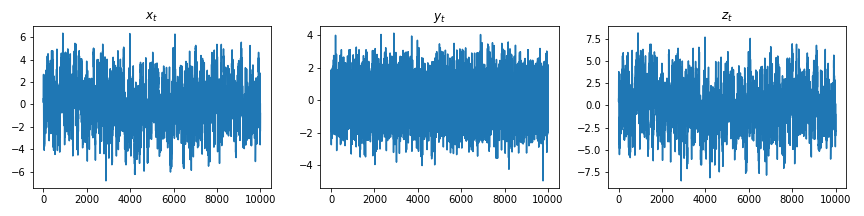
\includegraphics[width=\textwidth]{q4-a}
\caption{}
\label{4a}
\end{figure}
\end{proof}

\item
Compute and plot the (empirical) ACF and PACF for each process. Discuss.
\begin{proof}
Below is the code used to plot the ACF and PACF for each process. Figure \ref{4b} contains the sample autocorrelation and partial autocorrelation plots for the $x_t$, $y_t$ and $z_t$ processes, respectively. The first row of Figure \ref{4b} (AR(3)) displays a geometrically decaying autocorrelation function and a partial autocorrelation function that becomes zero after 3 lags. The second row of Figure \ref{4b} (MA(2)) has an autocorrelation function that becomes zero after two lags and partial autocorrelation function that tends to zero only gradually. The third row of Figure \ref{4b} (ARMA(3,2)) has an autocorrelation function resembling an AR(3) process since it decays geometrically and a partial autocorrelation function that resembles an MA(2) process because it converges to zero gradually. 
\begin{python3code}
fig, ax = plt.subplots(3,2,figsize=(12,8))
 
plot_acf(x, ax=ax[0,0]) 
plot_pacf(x, ax=ax[0,1]) 

plot_acf(y, ax=ax[1,0], title='')
plot_pacf(y, ax=ax[1,1], title='')

plot_acf(z, ax=ax[2,0], title='')
plot_pacf(z, ax=ax[2,1], title='')

plt.tight_layout()
plt.show()
\end{python3code}

\begin{figure}
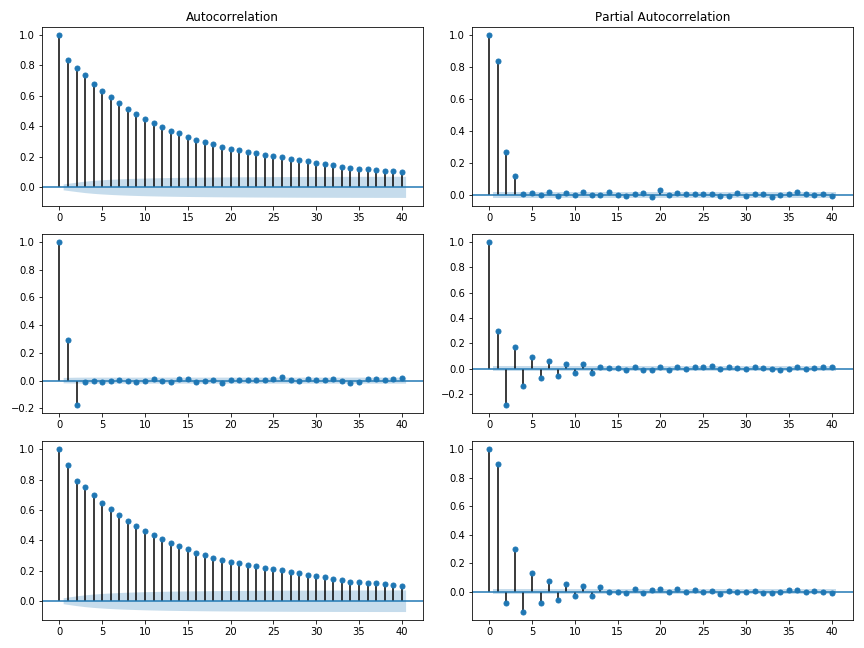
\includegraphics[width=\textwidth]{q4-b}
\caption{}
\label{4b}
\end{figure}
\end{proof}
\end{enumerate}



\end{document}
